\section{vLLM-FI Framework}
\label{sec:framework}

vLLM-FI extends the vLLM inference engine with runtime fault injection and reliability evaluation, reusing its native model execution and distributed runtime. First, we extend fault models for distributed LLM inference to account for computational workload and inter-device communication, enabling analysis of how faults affect inference outputs and downstream-task performance under different execution configurations. Second, we integrate fault configuration and target selection into vLLM's multi-process execution path to coordinate injection across distributed Workers and apply faults to the intended runtime tensors. Third, we implement GPU-resident, in-place bit-flip operators to reduce data transfers and injection overhead in large-scale fault-injection campaigns. The following subsections detail the system architecture, fault models, injection and evaluation workflow, and GPU implementation.

\subsection{System Architecture}
\label{subsec:architecture}

vLLM improves inference throughput and GPU memory utilization through continuous batching, PagedAttention-based KV-cache management, optimized computation kernels, quantized model execution, and distributed parallelism \cite{kwon2023efficient}. These capabilities make vLLM a suitable foundation for evaluating the reliability of practical LLM inference systems. However, they also make conventional model-level fault injection difficult to apply directly. A model may be partitioned differently according to the selected parallel strategy, and multiple parallel ranks are executed in separate Worker processes. Consequently, the model layers, parameters, intermediate results, and communication buffers to be injected are distributed across multiple devices and processes.

Figure~\ref{fig:vllmfi_architecture}(a) presents the overall vLLM-FI workflow, from fault configuration and task inputs through the vLLM-FI executor to evaluation. The input stage specifies the fault type, mode, target layer, and rank together with the model, parallelism, and inference settings. The executor integrates \textit{FaultConfig} with the native vLLM configuration and propagates it to the distributed Workers, while vLLM schedules task requests for token-level execution on the corresponding model partitions. The evaluation stage passes the resulting model outputs to \texttt{lm-evaluation-harness} for task-specific scoring, connecting configurable injection with downstream reliability assessment.

Figure~\ref{fig:vllmfi_architecture}(b) shows where the configured faults are applied within a Worker's model computation. The illustrated injector maps each configuration to a target in the attention or MLP block: a memory fault modifies the QKV projection weights, a compute fault perturbs an attention-computation result, and a communication fault modifies the output buffer associated with the MLP down projection before inter-device exchange. These examples connect the experiment-level settings in Fig.~\ref{fig:vllmfi_architecture}(a) to concrete injection locations in Fig.~\ref{fig:vllmfi_architecture}(b). At each selected location, the fault model determines the number of events, and the CUDA backend performs in-place bit flips on the GPU-resident tensor.

\subsection{Extended Fault Models}
\label{subsec:fault_models}

vLLM-FI supports memory, compute, and communication faults. In this work, these models target model weights, matrix-computation outputs, and software-visible communication buffers, respectively. As illustrated in Fig.~\ref{fig:three_fault_models}, injected weight corruption persists after loading, a compute fault perturbs an intermediate result during inference, and a communication fault affects data transferred between devices.

For each fault model, vLLM-FI provides both fixed-count and bit-error-rate modes. Fixed-count mode directly specifies the number of fault events. In bit-error-rate mode, the number of fault events is sampled from a Poisson distribution whose parameter is determined by the exposure associated with the selected fault model.

\begin{figure*}[t]
    \centering
    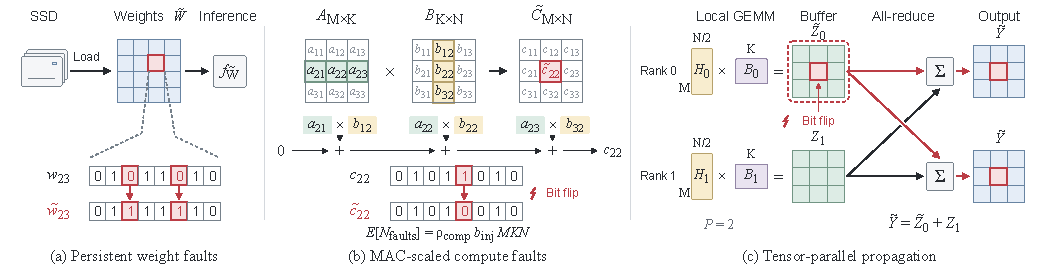
\includegraphics[width=\textwidth]{fault_models.pdf}
    \caption{\textbf{Model-visible fault abstractions supported by vLLM-FI.}
    Memory faults modify model weights during loading and persist throughout subsequent inference.
    Compute faults perturb intermediate results produced by matrix operations.
    Communication faults modify software-visible buffers associated with tensor-parallel collectives or pipeline-parallel transfers.}
    \label{fig:three_fault_models}
\end{figure*}


\subsubsection{Memory Faults}

Memory faults can corrupt data stored during LLM inference, including model weights, activations, and the KV cache. This work focuses on model weights because their long lifetime and repeated reuse allow corruption to affect many subsequent forward computations and decoding steps. A corrupted weight can therefore introduce persistent perturbations into inference and degrade downstream-task performance.

To evaluate this effect, vLLM-FI applies configurable bit flips to selected weight tensors as they are loaded into GPU memory. The modified values are retained and used in subsequent inference, allowing the evaluation workflow to measure their impact on model outputs. The loading stage serves as the injection point for establishing persistent weight corruption; the model does not restrict the physical occurrence of memory faults to model loading.

To determine the injection count, consider a weight tensor $\mathbf{W}$ containing $|\mathbf{W}|$ elements, each with a storage width of $b$ bits. Let $\rho_{\mathrm{mem}}$ denote the fault event rate per stored bit. The expected number of memory fault events is

\begin{equation}
    \lambda_{\mathrm{mem}}
    =
    |\mathbf{W}|b\rho_{\mathrm{mem}},
    \qquad
    N_{\mathrm{faults}}^{\mathrm{mem}}
    \sim
    \operatorname{Poisson}(\lambda_{\mathrm{mem}}).
    \label{eq:memory_exposure}
\end{equation}


\subsubsection{Compute Faults}

Compute faults model the effect of transient errors in arithmetic units on intermediate computation results \cite{ashraf2015understanding}. Existing model-level fault injection methods commonly estimate the number of compute faults according to the number of elements in an output tensor. However, the output size does not necessarily reflect the amount of computation required to produce that output.

For example, multiplying matrices with shapes $(a_1,a_2)$ and $(a_2,a_1)$ produces an output containing $a_1^2$ elements, but requires $a_1^2a_2$ multiply--accumulate operations. Increasing $a_2$ therefore increases the computational fault exposure without changing the number of output elements. This difference becomes more important for LLMs because of their large projection dimensions and the repeated execution of matrix operations during autoregressive decoding.

Following prior LLM reliability studies \cite{sun2025demystifying,sun2025ft2,xie2025realm}, vLLM-FI injects compute faults into the outputs of GEMM and related matrix operations. However, the number of faults is determined by the estimated multiply--accumulate workload rather than solely by the output-tensor size. Let $\mathcal{C}_{\mathrm{total}}$ be the estimated number of executed MAC operations and $b_{\mathrm{inj}}$ be the data width at the injection point. The compute exposure and the expected number of fault events are defined as

\begin{equation}
    \mathcal{E}_{\mathrm{comp}}
    =
    \mathcal{C}_{\mathrm{total}}b_{\mathrm{inj}},
    \qquad
    \lambda_{\mathrm{comp}}
    =
    \rho_{\mathrm{comp}}\mathcal{E}_{\mathrm{comp}},
    \label{eq:compute_exposure}
\end{equation}

\begin{equation}
    N_{\mathrm{faults}}^{\mathrm{comp}}
    \sim
    \operatorname{Poisson}(\lambda_{\mathrm{comp}}),
    \label{eq:compute_poisson}
\end{equation}

where $\rho_{\mathrm{comp}}$ denotes the compute-fault event rate per exposed bit operation.

Algorithm~\ref{alg:mac_estimation} summarizes the runtime MAC estimation procedure. Linear projections use their executed batch size, input dimension, and output dimension. Fused modules, such as \texttt{gate\_up\_proj}, are treated according to the dimensions of the fused runtime operator. Attention computation is estimated using the sequence metadata provided by vLLM, allowing the framework to distinguish prefill from decode and to account for the effective number of query--key pairs under causal attention. The current model excludes non-MAC operations such as Softmax, normalization, rotary position encoding, and data movement.

\begin{algorithm}[t]
\footnotesize
\DontPrintSemicolon
\SetAlgoVlined
\SetInd{0.35em}{0.75em}
\SetAlgoNlRelativeSize{-1}
\caption{Runtime MAC Estimation}
\label{alg:mac_estimation}
\KwIn{Projection shapes $\mathcal{P}$; query offsets $\mathbf{s}$; context lengths $\boldsymbol{\ell}$; query-head count $N_q$; head dimension $D_h$}
\KwOut{Estimated MAC count $\mathcal{C}_{\mathrm{total}}$}

$\mathcal{C}_{\mathrm{proj}} \leftarrow 0$;

\ForEach{$(N,D_{\mathrm{in}},D_{\mathrm{out}}) \in \mathcal{P}$}{
    $\mathcal{C}_{\mathrm{proj}}
    \leftarrow
    \mathcal{C}_{\mathrm{proj}}
    +
    ND_{\mathrm{in}}D_{\mathrm{out}}$;
}

$\mathcal{C}_{\mathrm{attn}} \leftarrow 0$;

\For{$i \leftarrow 0$ \KwTo $|\boldsymbol{\ell}|-1$}{
    $L_q \leftarrow \mathbf{s}[i+1]-\mathbf{s}[i]$;

    $L_{\mathrm{kv}} \leftarrow \boldsymbol{\ell}[i]$;

    \eIf{$L_q>1$}{
        $N_{\mathrm{eff}}
        \leftarrow
        L_q\left(
        L_{\mathrm{kv}}
        -
        \frac{L_q-1}{2}
        \right)$;
    }{
        $N_{\mathrm{eff}}
        \leftarrow
        L_qL_{\mathrm{kv}}$;
    }

    $\mathcal{C}_{\mathrm{attn}}
    \leftarrow
    \mathcal{C}_{\mathrm{attn}}
    +
    2N_qN_{\mathrm{eff}}D_h$;
}

$\mathcal{C}_{\mathrm{total}}
\leftarrow
\mathcal{C}_{\mathrm{proj}}
+
\mathcal{C}_{\mathrm{attn}}$;

\Return{$\mathcal{C}_{\mathrm{total}}$};
\end{algorithm}


\subsubsection{Communication Faults}

Communication faults model errors affecting data exchanged between devices during distributed inference. vLLM-FI targets software-visible communication buffers in both tensor-parallel and pipeline-parallel execution. For tensor parallelism, faults are injected into buffers associated with collective operations such as All-Reduce. For pipeline parallelism, faults are injected into activation buffers transferred between adjacent pipeline stages.

At a selected communication location, let $\mathbf{B}$ denote the communication buffer, $|\mathbf{B}|$ the number of elements in that buffer, $b$ the number of bits per element, and $\rho_{\mathrm{comm}}$ the communication-fault event rate. The number of injected communication faults is sampled as

\begin{equation}
    \lambda_{\mathrm{comm}}
    =
    |\mathbf{B}|b\rho_{\mathrm{comm}},
    \qquad
    N_{\mathrm{faults}}^{\mathrm{comm}}
    \sim
    \operatorname{Poisson}(\lambda_{\mathrm{comm}}).
    \label{eq:comm_exposure}
\end{equation}

The selected bits are modified before the corresponding collective operation or pipeline-stage transfer. The corrupted buffer therefore participates in subsequent communication and computation, allowing the resulting error to propagate across devices. This abstraction models corruption that is visible in the software communication path. Low-level link protocols, retransmission mechanisms, and internal interconnect behavior remain outside the scope of vLLM-FI.


\subsection{vLLM-Native Fault Injection and Evaluation}
\label{subsec:runtime_injection}

Introducing an independent fault configuration into vLLM is non-trivial. To reach the actual injection locations, a newly defined configuration must pass through the Engine, Executor, Worker processes, ModelRunner, and runtime layer implementations. vLLM-FI addresses this problem by implementing \textit{FaultConfig} as a sub-configuration of \textit{VllmConfig}. The fault configuration can therefore reuse the native vLLM configuration-propagation path and reach the corresponding injection locations inside each Worker. Each Worker evaluates the fault-activation settings in \textit{FaultConfig} against its current device, rank, pipeline stage, model module, fault type, and execution conditions, and activates the corresponding injector when the configured conditions are satisfied. In this way, \textit{FaultConfig} provides configuration-level support for distributed fault injection without introducing an independent cross-process control path.

Weight fault injection additionally requires resolving the runtime parameter held by each Worker. If injection were performed by traversing the entire model after model loading, the target specified in the fault configuration would have to be remapped to the runtime parameters held by different Workers under the selected parallel configuration. To avoid implementing this additional mapping procedure, vLLM-FI embeds weight fault injection into the weight-loading methods of vLLM linear layers. At this location, the target model layer and the parameter currently being loaded by the Worker are directly available. Without tensor parallelism, the injector operates on the complete loaded parameter. Under tensor parallelism, it operates on the weight shard selected for the current rank. Under pipeline parallelism, the weight-loading method is executed only for the model layers assigned to the current pipeline stage. Quantized weights, including packed \texttt{qweight} parameters, follow the same injection path and are distinguished through an additional check of the parameter name and storage representation.

Unlike weight faults, compute and communication faults occur during runtime inference rather than during model loading. vLLM-FI therefore places their injection sites in the forward execution paths of the corresponding runtime layers. A compute fault is triggered after the selected matrix operation produces its output. A communication fault modifies the corresponding communication buffer before a tensor-parallel collective or a pipeline-stage transfer. Because these injection mechanisms execute inside the Worker, they directly operate on the runtime tensors produced under the current device and parallel context. Together with the distributed activation settings provided by \textit{FaultConfig}, the runtime injection mechanisms support tensor parallelism, pipeline parallelism, and their combined configurations. Placing the injection sites in shared runtime layer definitions also allows the same mechanism to be reused across supported model architectures.

Reliability evaluation across different models, datasets, and inference configurations otherwise requires repeated implementation of dataset loading, model invocation, output processing, and task-specific metric calculation. To reduce this repeated work, vLLM-FI adapts \texttt{lm-evaluation-harness} to support \textit{FaultConfig}. The modified interface passes \textit{FaultConfig}, together with the existing vLLM parameters, to the vLLM backend. It constructs benchmark inputs, executes inference under the specified fault configuration, collects the fault-affected outputs, and computes the native metrics of the selected downstream task. This integration provides an end-to-end workflow from distributed fault injection to standardized task-level reliability evaluation.


\subsection{GPU-Resident In-Place Bit-Flip Operator}
\label{subsec:cuda_operator}

Existing model-level fault injection tools for CNNs and conventional DNNs generally prioritize portable and extensible implementations based on PyTorch-level operations \cite{mahmoud2020pytorchfi,huang2024mrfi}. Their typical experiments inject only one or a small number of faults during each forward pass. Under such workloads, the additional injection overhead is relatively limited, and the performance benefit of developing and maintaining a dedicated CUDA operator is therefore less significant.

This design trade-off changes for LLM fault injection. Autoregressive generation repeatedly executes model layers across multiple decoding steps, causing runtime injection sites to be triggered many times. Moreover, vLLM-FI determines the number of fault events according to the configured error rate and compute exposure, such that more faults must be processed as the target workload or error rate increases. With CPU-assisted bit modification, host--device transfers and synchronization are repeatedly introduced across model layers and decoding steps, while a larger number of faults also increases the transferred data volume and host-side bit-manipulation workload. As shown in Fig.~\ref{fig:controlled_injection_runtime}, the runtime difference between CPU-assisted and CUDA-based injection is relatively small at low error rates but grows rapidly as the error rate and the number of injected faults increase. GPU-resident batched in-place modification therefore changes from an optional optimization for conventional workloads into a practical requirement for efficient LLM fault injection.

To eliminate this CPU round trip, vLLM-FI implements a custom CUDA bit-flip operator that directly modifies target tensors residing in GPU memory. Given a target tensor and the fault injection parameters, the operator performs target-position selection, bit-mask construction, and binary-data modification on the GPU without copying the selected values to the CPU. This design confines the data manipulation introduced by fault injection to the GPU and allows multiple fault events within an injection call to be processed in parallel.

Moving bit flipping to the GPU also requires adapting the injection procedure to different data representations. Full-precision and quantized data types have different storage widths and encoding layouts and therefore cannot be modified using a single uniform bit-manipulation procedure. vLLM-FI implements data-type-specific bit operations for each supported representation.

For each fault event, the CUDA operator independently samples an element from the target tensor and selects one or two distinct bit positions permitted by the configured bit-selection policy. It then constructs an XOR mask from the selected positions and applies the mask to the underlying binary representation of the target element.

The eligible bit positions are determined jointly by the tensor data type and the configured bit-selection policy. Full-width injection supports FP64, FP32, FP16, BF16, INT8, UINT8, INT16, INT32, INT64, FP8 E5M2, and FP8 E4M3FN. For FP16, BF16, and FP8 values, field-specific injection can further restrict faults to the sign, exponent, or mantissa field. Through type-specific dispatch over the underlying storage representation, the same operator can directly process full-precision weights and activations, quantized weights, and other intermediate representations without first converting them to a common CPU format.

% \section{vLLM-FI Framework}
% \label{sec:framework}

% This section presents the design and implementation of vLLM-FI. It focuses on how the tool performs configurable fault injection on the native vLLM execution path. We first describe the constraints imposed by the multi-process runtime and the overall architecture. The remaining subsections present fault models, cross-process configuration propagation, runtime target selection, GPU-resident bit flipping, and automated reliability evaluation.

% \subsection{Design Goals and System Architecture}
% \label{subsec:architecture}

% vLLM improves inference throughput and GPU memory utilization through continuous batching, PagedAttention-based KV-cache management, optimized computation kernels, and distributed parallel execution \cite{kwon2023efficient}. However, the runtime architecture supporting these optimizations complicates conventional hook-based fault injection. Unlike a typical PyTorch program, which stores the model object in a single process, vLLM executes models in Worker processes launched by a scheduling process. Consequently, model instances and layer objects reside inside the Workers and are not directly accessible from the entry process. External forward hooks therefore cannot reliably locate or modify a target layer. Distributed execution further partitions parameters and intermediate results across ranks. vLLM-FI must therefore propagate fault configurations across process boundaries and perform injection inside the appropriate Worker at the correct rank and runtime location.

% vLLM-FI addresses these constraints through a configuration-driven injection path integrated into the native vLLM runtime. For each experiment, the system receives a set of inference requests, a vLLM execution configuration, and a \textit{Fault Config}. The vLLM execution configuration specifies the model, quantization method, parallel configuration, and inference parameters, whereas the \textit{Fault Config} specifies the fault type, injection target, and injection strength. During execution, the fault configuration is propagated to the Workers, where vLLM-FI applies controlled perturbations to selected model weights, operator outputs, or communication buffers. The resulting inference outputs retain the format expected by downstream task evaluators.

% Three goals guide this architecture: configuration simplicity, efficient injection, and precise runtime targeting. First, vLLM-FI manages the \textit{Fault Config} together with the native vLLM execution parameters and automatically handles its propagation across processes. Second, it modifies GPU-resident target tensors in place, avoiding CPU copies and host--device transfers introduced solely by fault injection. Third, it resolves injection targets using the runtime representations and execution locations employed by vLLM, including quantized tensors, fused operators, and rank-local data. These extensions do not alter model partitioning, Worker launch, device placement, or scheduling, which remain under the control of vLLM.

% \begin{figure*}[t]
%     \centering
%     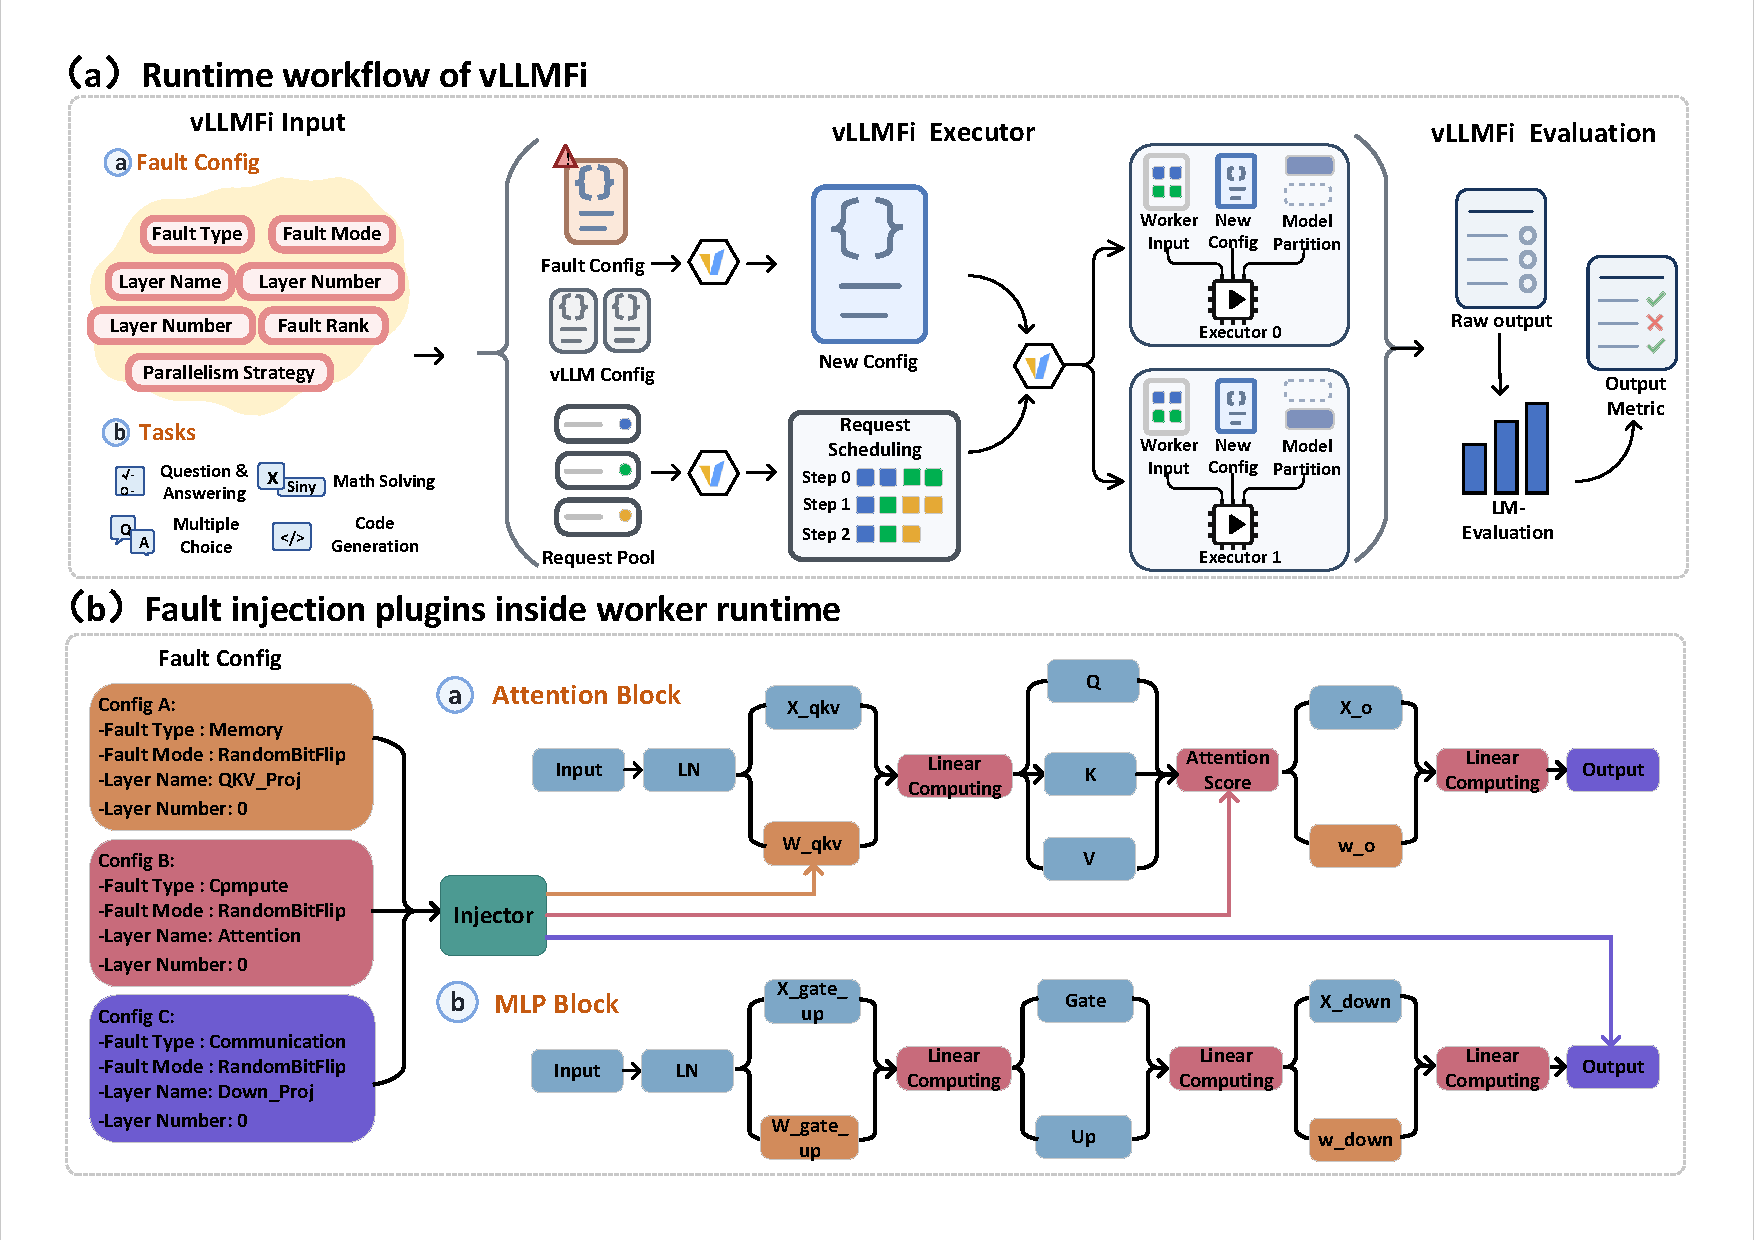
\includegraphics[width=0.82\textwidth]{vLLMFI.pdf}
%     \caption{\textbf{Overview of the vLLM-FI architecture and execution workflow.}
%     vLLM schedules inference requests from the evaluation dataset, while Fault Config is integrated with the native configuration and propagated to the Workers. Worker-side injectors perturb selected GPU-resident tensors during inference, and \texttt{lm-evaluation} evaluates the resulting outputs.}
%     \label{fig:vllmfi_architecture}
% \end{figure*}

% Figure~\ref{fig:vllmfi_architecture} illustrates the configuration-driven architecture and execution workflow of vLLM-FI. The evaluation dataset and Fault Config are provided as system inputs, while vLLM schedules the inference requests generated from the dataset. Fault Config is integrated with the native vLLM execution configuration to form a unified runtime configuration, which is then propagated to the Workers through the Executor. During model inference, each Worker activates the appropriate fault injector according to the fault type, injection target, and injection strength specified in Fault Config. The fault-affected model outputs are subsequently returned to lm-evaluation, which evaluates the injection results using the task-specific metrics associated with the dataset.

% \subsection{Fault Models and Injection-Strength Modeling}
% \label{subsec:fault_models}

% vLLM-FI defines memory, compute, and communication faults on model weights, operator results, and communication buffers. The framework supports fixed-count and bit error rate modes.Fixed-count mode specifies the number of fault events. BER mode derives the Poisson parameter $\lambda$ from the exposure of the target object. The following subsections define the exposure and event count for each fault model.

% \begin{figure*}[t]
%     \centering
%     \subfloat[Memory fault during weight loading.\label{fig:fault_memory}]{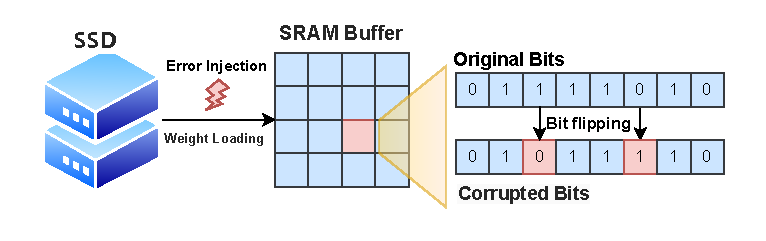
\includegraphics[width=0.30\textwidth]{memory_error.drawio.pdf}}
%     \hfill
%     \subfloat[Compute fault in an operator result.\label{fig:fault_compute}]{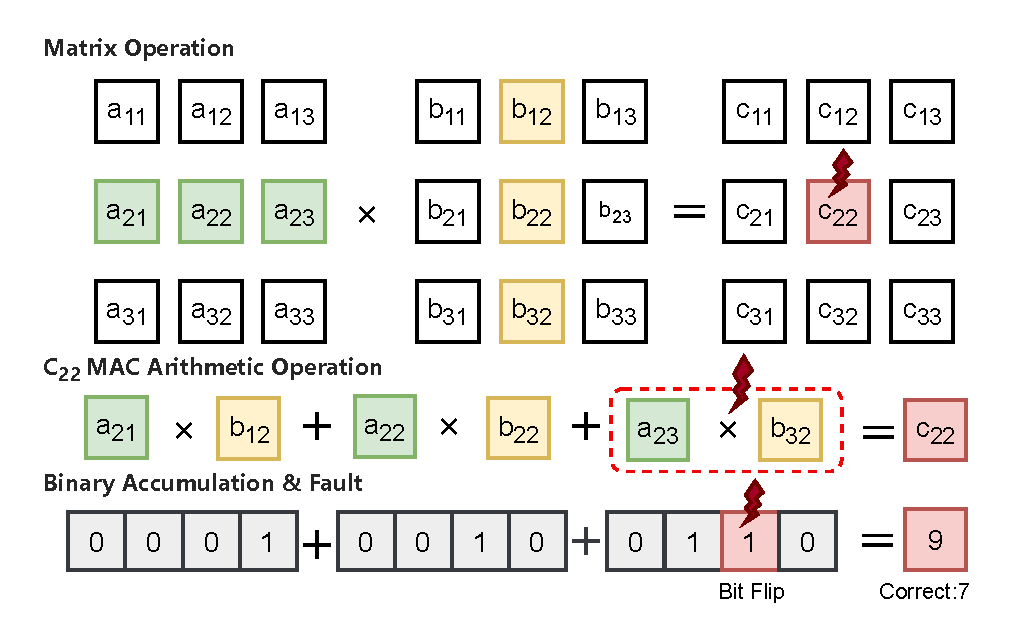
\includegraphics[width=0.30\textwidth]{compute_error.drawio.pdf}}
%     \hfill
%     \subfloat[Communication fault before a collective.\label{fig:fault_comm}]{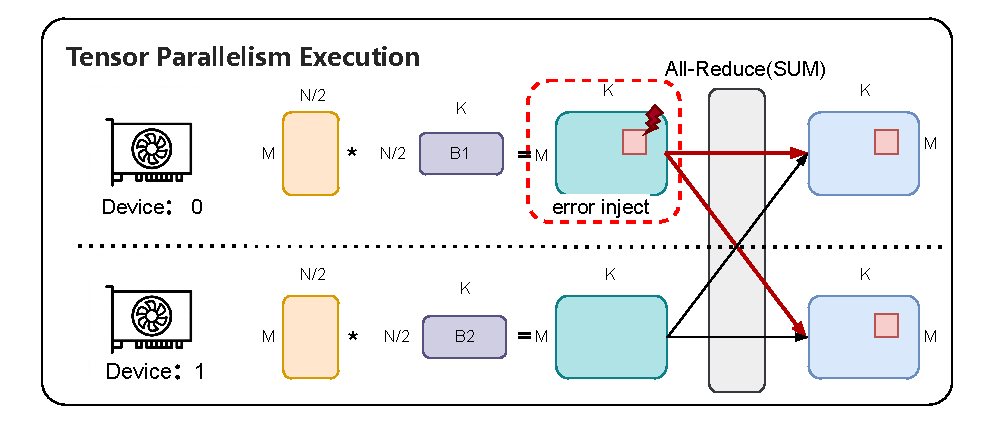
\includegraphics[width=0.30\textwidth]{communication_error_v2.drawio.pdf}}
%     \caption{Model-visible fault abstractions in vLLM-FI. A weight perturbation persists after loading. A compute perturbation changes an intermediate result. A communication perturbation is applied to a local buffer before collective communication and may propagate through data exchange or aggregation.}
%     \label{fig:three_fault_models}
% \end{figure*}

% \subsubsection{Memory Faults}

% Memory faults model weight corruption during storage or loading. Error-correcting code can detect or correct many single-bit errors. Uncorrectable multi-bit errors may still cause silent data corruption \cite{hsiao2023silent,papadimitriou2021demystifying,jiao2025large}. vLLM-FI injects random double-bit flips while weights enter the GPU execution path. A modified weight remains corrupted during subsequent forward computations and autoregressive decoding.

% For a weight tensor $\mathbf{W}$ with $|\mathbf{W}|$ elements and a storage width of $b$ bits per element, let $\rho_{\mathrm{mem}}$ be the fault-event rate per stored bit. The fault count is
% \begin{equation}
%     \lambda_{\mathrm{mem}}=|\mathbf{W}|b\rho_{\mathrm{mem}},
%     \qquad
%     N_{\mathrm{faults}}^{\mathrm{mem}}
%     \sim \operatorname{Poisson}(\lambda_{\mathrm{mem}}).
%     \label{eq:memory_exposure}
% \end{equation}

% \subsubsection{Compute Faults}

% Compute faults model the effect of transient errors in arithmetic units on intermediate results \cite{ashraf2015understanding}. Following prior LLM reliability studies \cite{sun2025demystifying,sun2025ft2,xie2025realm}, vLLM-FI maps them to bit perturbations in GEMM and related matrix-computation outputs.

% Compute exposure is defined by the multiply--accumulate (MAC) workload represented by the target operators. Let $\mathcal{C}_{\mathrm{total}}$ be the estimated MAC count and $b_{\mathrm{inj}}$ the data width at the injection point. The bit-level compute exposure and expected event count are
% \begin{equation}
%     \mathcal{E}_{\mathrm{comp}}=\mathcal{C}_{\mathrm{total}}b_{\mathrm{inj}},
%     \qquad
%     \lambda_{\mathrm{comp}}=\rho_{\mathrm{comp}}\mathcal{E}_{\mathrm{comp}},
%     \label{eq:compute_exposure}
% \end{equation}
% \begin{equation}
%     N_{\mathrm{faults}}^{\mathrm{comp}}
%     \sim \operatorname{Poisson}(\lambda_{\mathrm{comp}}).
%     \label{eq:compute_poisson}
% \end{equation}

% Algorithm~\ref{alg:mac_estimation} summarizes the runtime MAC estimate. Linear projections use their executed input and output dimensions. Fused modules, such as \texttt{gate\_up\_proj}, use the dimensions of the fused runtime operator. Attention uses sequence metadata supplied by vLLM to distinguish prefill from decode. The current estimate excludes non-MAC operations, including Softmax, normalization, rotary position encoding, and data movement.

% % This algorithm is intentionally single-column.
% \begin{algorithm}[t]
% \footnotesize
% \DontPrintSemicolon
% \SetAlgoVlined
% \SetInd{0.35em}{0.75em}
% \SetAlgoNlRelativeSize{-1}
% \caption{Runtime MAC Estimation}
% \label{alg:mac_estimation}
% \KwIn{Projection shapes $\mathcal{P}$; query offsets $\mathbf{s}$; context lengths $\boldsymbol{\ell}$; query-head count $N_q$; head dimension $D_h$}
% \KwOut{Estimated MAC count $\mathcal{C}_{\mathrm{total}}$}
% $\mathcal{C}_{\mathrm{proj}} \leftarrow 0$;
% \ForEach{$(N,D_{\mathrm{in}},D_{\mathrm{out}}) \in \mathcal{P}$}{
%     $\mathcal{C}_{\mathrm{proj}} \leftarrow \mathcal{C}_{\mathrm{proj}}+ND_{\mathrm{in}}D_{\mathrm{out}}$;
% }
% $\mathcal{C}_{\mathrm{attn}} \leftarrow 0$;
% \For{$i \leftarrow 0$ \KwTo $|\boldsymbol{\ell}|-1$}{
%     $L_q \leftarrow \mathbf{s}[i+1]-\mathbf{s}[i]$;
%     $L_{\mathrm{kv}} \leftarrow \boldsymbol{\ell}[i]$;
%     \eIf{$L_q>1$}{
%         $N_{\mathrm{eff}} \leftarrow L_q\left(L_{\mathrm{kv}}-\frac{L_q-1}{2}\right)$;
%     }{
%         $N_{\mathrm{eff}} \leftarrow L_qL_{\mathrm{kv}}$;
%     }
%     $\mathcal{C}_{\mathrm{attn}} \leftarrow \mathcal{C}_{\mathrm{attn}}+2N_qN_{\mathrm{eff}}D_h$;
% }
% $\mathcal{C}_{\mathrm{total}} \leftarrow \mathcal{C}_{\mathrm{proj}}+\mathcal{C}_{\mathrm{attn}}$;
% \Return{$\mathcal{C}_{\mathrm{total}}$};
% \end{algorithm}

% \subsubsection{Communication Faults}

% Communication faults model errors during data exchange in multi-device inference. vLLM-FI flips bits in a local communication buffer before a collective call. Corrupted data then participates in operations such as All-Reduce and may propagate to other ranks.

% Communication exposure is derived from the transferred data volume. Consider a Ring All-Reduce with tensor-parallel size $P$ and a communication tensor containing $N_{\mathrm{elem}}$ elements. Its Reduce-Scatter and All-Gather phases produce the following per-rank element volume:
% \begin{equation}
%     V_{\mathrm{comm}}=\frac{2(P-1)}{P}N_{\mathrm{elem}}.
%     \label{eq:comm_volume}
% \end{equation}
% For a communication width of $b$ bits and a target rate $\rho_{\mathrm{comm}}$, vLLM-FI samples
% \begin{equation}
%     \lambda_{\mathrm{comm}}=V_{\mathrm{comm}}b\rho_{\mathrm{comm}},
%     \qquad
%     N_{\mathrm{faults}}^{\mathrm{comm}}
%     \sim \operatorname{Poisson}(\lambda_{\mathrm{comm}}).
%     \label{eq:comm_exposure}
% \end{equation}
% This model separates communication-path exposure from an equal-sized local tensor perturbation. It captures the software-visible buffer corruption. Link protocols, retransmission, and internal interconnect behavior remain outside its scope.

% \subsection{Configuration-Driven Runtime Injection}
% \label{subsec:runtime_injection}

% Fault Config extends the native vLLM execution configuration with controlled fault-injection metadata. It records the fault type, fault mode, target rank, injection strength and random seed. The evaluation dataset and Fault Config are provided to vLLM-FI as system inputs. vLLM schedules the inference requests derived from the dataset, while vLLM-FI integrates Fault Config with the native execution settings to form a unified runtime configuration. The Executor then propagates this configuration to the Workers.

% Within each Worker, vLLM-FI registers candidate injection sites along the weight-loading, operator-computation, and collective-communication paths. At each candidate site, the Worker checks the current module, execution stage, and local rank against Fault Config. When all conditions match, the Worker passes the target tensor and injection parameters to the custom CUDA bit-flip operator, which modifies the selected GPU-resident tensor in place.

% Rank selection supports a single rank, a list of ranks, or all ranks. Each Worker compares its local rank with the configured target set. Single-rank mode enables injection only in the selected Worker, while multi-rank mode enables injection in the listed Workers. All-rank mode permits injection in every Worker that satisfies the configured module and execution-stage conditions.

% The mechanism operates within the native parallel context created by vLLM and does not alter model partitioning, device placement, or scheduling. Under tensor parallelism, a matching Worker modifies the local parameter shard, intermediate tensor, or communication buffer that it owns. Under pipeline parallelism, injection is activated only in the stage that executes the target layer and satisfies the rank condition.

% For communication faults, the injection scope covers all inter-GPU communication sites, including collective communication within tensor-parallel layers and activation transfers at pipeline-stage boundaries. Within each communicated tensor, fault locations are sampled according to the configured bit error rate. After inference, the fault-affected outputs are returned to \texttt{lm-evaluation} for task-specific evaluation.
% \subsection{GPU-Resident In-Place Bit-Flip Operator}
% \label{subsec:cuda_operator}

% vLLM-FI uses a custom CUDA operator to modify selected GPU-resident tensors in place. The operator receives a tensor pointer and the injection parameters, and directly modifies the underlying binary storage without creating a CPU copy.

% For each fault event, the operator samples a tensor element and selects one or two distinct bit positions permitted by the configured policy. It constructs an XOR mask from the selected positions and applies the mask to the stored binary representation of the element. The eligible bit positions are determined by the tensor data type and the bit-selection policy. Full-width mode supports FP64, FP32, FP16, BF16, INT8, UINT8, INT16, INT32, INT64 , FP8 E5M2 and FP8 E4M3FN. Field-specific mode restricts faults in FP16, BF16, and FP8 values to the sign, exponent, or mantissa fields.

% Updates are performed using atomic XOR operations. For 32-bit and 64-bit storage words, the operator applies the mask directly to the corresponding word. Since CUDA does not provide native atomic XOR operations for 8-bit or 16-bit values, vLLM-FI maps each target value to its enclosing aligned 32-bit word. It then shifts the mask according to the byte or half-word offset and performs a 32-bit atomic XOR operation. This procedure preserves the remaining bits in the storage word and prevents lost updates when multiple threads concurrently access the same word.
% The kernel assigns scheduled fault events to CUDA threads. The element and bit positions for each event are determined by a base random seed and the thread index. The kernel executes on the caller-provided CUDA stream without introducing explicit device-wide synchronization. Identical configurations, random seeds, and execution conditions reproduce the same injection positions. Section 5 evaluates the end-to-end runtime overhead.

% \subsection{Automated End-to-End Reliability Evaluation}
% \label{subsec:evaluation_loop}

% Fault injection produces perturbed outputs. A complete reliability study must also load tasks, construct inputs, run inference, score outputs, and aggregate results. Separate scripts for these steps increase the effort required to add a task or fault configuration. vLLM-FI integrates with \texttt{lm-evaluation-harness} to expose one evaluation workflow.

% Users select the model, downstream task, vLLM settings, and Fault Config through a common command-line entry. The system initializes the model, propagates the fault configuration, triggers runtime injection, collects outputs, and invokes the task evaluator. Changing the fault model, target, or task requires configuration changes rather than new model-loading, trigger, or scoring code.

% The task evaluator first produces the native benchmark metric. The result-processing stage aggregates repeated runs and computes normalized values against a fault-free baseline. This configuration-driven loop simplifies batch experiments and records the information required for reproduction. Section~\ref{sec:experimental_setup} defines the common workloads and evaluation protocol.
